\cotefile{53}
\scanpage{2}
Groupes algébriques.
% margin note written sideways
\margin{Groupes Alg\unsure{e|é}briques}
% archive sheet number: 1

\scanpage{3}
\deleted{\uline{\unsure{Déf|Dèf}}}\quad
\deleted{\uline{Prop} $G\times G\xrightarrow{p}G$ ouvert}

\deleted{\uline{Cor.} Si $P$ un \inserted{\unsure{pr.|ps.}} torseur sous $G$ ($G\times P\xrightarrow[\unsure{1|\vert}]{\sim}P\times P$\inserted{$(g,x)\mapsto(gx,x)$}) alors $\pi:G\times P\longrightarrow P$ ouvert}

\deleted{\unsure{Lemme|lemme}}\quad
\deleted{\uline{Lemme} Soit $X$ schéma sur lequel $G$ opère. Conditions \unsure{équivaltes|équivalentes}}

\deleted{a) $\forall\,S$ sur $k$, et section \deleted{\unsure{un|une}} $a$ de $X_S$ sur $S$, le morphisme $G_S\longrightarrow X_S$, $g\mapsto ga$, est ouvert (resp. ouvert surjectif)}

\deleted{b) Le morphisme \inserted{$\unsure{a_x|a.}:(g,x)\mapsto(gx,x)$} $G\times X\longrightarrow X\times X$ est \deleted{\unsure{univ.}} ouvert\inserted{ univ. sur $X$} (resp. univ. ouvert et surjectif)}

\deleted{c) $\exists$ un $S$ sur $k$, $S\ne\varnothing$, et une \deleted{\unsure{immersion}} section $a$ de $X_S$ sur $S$, tels que}

\uline{Prop} $G$ \inserted{\unsure{schém. en|schém. en.}} groupes sur $S$. $G$ séparé $/S$ ssi section unité est \uline{fermée}

\uline{Cor} $G$ groupe sur corps. Alors $G$ séparé

\uline{Prop} $G$ \unsure{gpe|grp} sur un corps. Alors $p:G\times G\longrightarrow G$ \inserted{univ.} ouvert. Plus \unsure{gén|gén.}, \deleted{\unsure{Cor|Cor.}}\inserted{si} $\deleted{P}X$ \inserted{\unsure{ps|pr}} torseur sous $G$. Alors $G\times\deleted{P}X\xrightarrow{\pi}\deleted{P}X$ est \inserted{univ.} ouvert

\deleted{\uline{Lemme} Soit $G$ opérant sur $X$. Soit \deleted{\illegible{1}} s'il $\exists$ un corps $k'/k$ et $a\in X(k')$ tel que $G_{k'}\longrightarrow X_{k'}$, $g\longmapsto ga$ est ouvert \inserted{univ. $/k'$} (resp. \unsure{univ.} surjectif) c'est vrai pour tt autre p$^{\mathrm{t}}$ de $X$ \unsure{à|:} \unsure{valeurs|valeur} dans un $k''/k$, et \unsure{m.|un} à valeur \unsure{dans|sur} un $S$.}

\deleted{On dit que $X$ est un espace homogène.}

\uline{Prop} \deleted{Supposons que $G\times X\xrightarrow{\pi}X$ soit ouvert (p. ex. $\deleted{P}X$ un \unsure{ps.} torseur),} Alors pour tt $U\subset G$, $V\subset \deleted{P}X$, $U$;$V$ ouverts, \unsure{\ldots}

a) $U.V$ ouvert si $\pi$ ouvert (p ex. $\deleted{P}X$ un ps. tors.)

% slanted
\margin{\unsure{comprendre|comprends} l'\uline{\unsure{évid.}} de c.}
b) $U.V$ stable par $G_0$ \deleted{\unsure{générisation|translation}}

c) $UV$ stable par spécialisation \deleted{\unsure{pour}} (\inserted{si} \deleted{$\pi$ est \unsure{générisant})} \inserted{les $\varphi_{\unsure{x|{}}}:G_{k'}\longrightarrow X_{k'}$ générisants} $x\in X(k')$) \deleted{p. ex. ouverts)}

c$'$) Si $U,V$ \unsure{qu. cpcts|qu. cpts} (et $X$ \inserted{qu} séparé), ou $\unsure{X|k}$ loc. \unsure{noeth|nœth}, $U\times V$ est fermé.

\uline{Cor} Supposons \deleted{\unsure{qu|que}} $\pi:G\times X\longrightarrow X\times X$ ouvert\inserted{ et $X$ quasi-sép.} \inserted{(p. ex $X$ un ps. torseur)}. Alors $X$ est réunion de parties \unsure{qu. cpctes|qu. cptes} \deleted{ouvertes}\inserted{$W_i$} qui sont à la fois ouvertes, fermées, et quasi-compactes [donc stables par $G^0$]. En particulier, les comp. connexes de $X$ sont quasi-compactes.

\margin{?}(Cor.\unsure{?}) Les composantes connexes de $X$ sont les comp irréductib\unsure{les}
% archive sheet number: 2

\scanpage{4}
% Broad oblique strokes cancel the upper-left working, including its diagram.
\[
\begin{aligned}
 &\deleted{\unsure{\mu_p|\mathbb{H}_p}}\quad \deleted{G}\quad \deleted{G^0}\qquad \deleted{\unsure{k[[t|k[[+}}\\
 &\hspace{2em}\deleted{k}\qquad \deleted{\deleted{\unsure{\mathcal O|G}}\unsure{k_{\mathrm{red}}|G_{\mathrm{red}}}}
 \hspace{9em}\deleted{\Delta_0\unsure{\ni|\supset|\Rightarrow}\Delta}
\end{aligned}
\]

\[
\begin{aligned}
 \deleted{\unsure{\mathcal R|R}=\unsure{\mathbb A b|\mathrm{Ab}}(\unsure{\mathcal C|C})^{\mathrm{op}}}
 &\quad\deleted{\unsure{\overline{\mathcal R}|\overline{R}}}
 \qquad\deleted{\sigma=\{G^{\unsure{n|h}}\}}\\
 \deleted{\unsure{\prime\prime|\prime}}\quad &\deleted{G^n\unsure{-|\longrightarrow}G^m}\\
 \deleted{\mathbb A b(\mathcal C)}\quad &\deleted{G^n\longrightarrow G}
\end{aligned}
\]

\diagram{\begin{tikzcd}[ampersand replacement=\&,row sep=small,execute at end picture={\draw[gray] (\tikzcdmatrixname-3-1.south west) -- (\tikzcdmatrixname-1-1.north east);\draw[gray] (\tikzcdmatrixname-3-2.south west) -- (\tikzcdmatrixname-1-3.north east);}]
{\deleted{\text{\uuline{$\mathrm{Hom}$}}'(\text{\textcircled{$\sigma$}},(\mathrm{ENS})\unsure{)|{}}}}\arrow[dd,bend left=5] \& \& {\deleted{\unsure{FN|EN}}}\\
{} \& {\deleted{\text{\unsure{topos|transp.}}}}\arrow[l] \& {}\\
{\deleted{(\mathrm{ENS})}}\arrow[uu,bend left=20] \& {\deleted{\unsure{\mathrm{sp}|\mathrm{sr}}\;\mathcal R\Rightarrow}} \& {}
\end{tikzcd}}

% The following right-hand block has three diagonal cancellation strokes.
\deleted{\deleted{Soit} Disons posant $(C'_i,\lambda'_i)=(C_{\psi(i)},\lambda_{\psi(i)})$, on voit que \deleted{$C'_i$ est tel que}}

\diagram{\begin{tikzcd}[ampersand replacement=\&,row sep=small,execute at end picture={\draw[gray] (\tikzcdmatrixname-2-1.south west) -- (\tikzcdmatrixname-1-2.north west);}]
{\deleted{C'_{i\deleted{\unsure{+1|+n}}}}}\arrow[r] \& {\deleted{C'_{i+1}}}\\
{\deleted{C_{\psi(i)}}}\arrow[u,equal] \& {\deleted{C_{\psi(i+1)}=g\psi(i)}}\arrow[u,equal]
\end{tikzcd}}

\deleted{est $\lambda'_i$-préexact. Donc si $\omega'$ est le plus petit ordinal $<\omega$ tel que $\omega'$ soit de \unsure{cardinalité|cofinalité} $\pi'$, on voit que \deleted{\unsure{si}} (par le \inserted{\unsure{=}} lemme du 1°) $\lambda_{\omega}^{\prime\unsure{\star|{}}}$ est exact dans $C'_{\omega}$, \deleted{donc $g(\omega)=$} cqfd.}

\margin{\uuline{\unsure{Lemme}}}
\uline{Dém} prop \qquad a) est trivial \qquad\unsure{$\sim$|v}

b) \deleted{Soit $x\in$} OPS $U,V\ne\varnothing$, \deleted{\illegible{1} si pour} on est ramené à prouver que si \deleted{$x\in W=U.V\quad W(k)$} $x=u_0v_0$ \inserted{$(u_0\in U(k),v_0\in V(k))$} \deleted{(tel à $U.V$)} alors l'image inverse de $\unsure{UV|U.V}$ dans $G$ par $G\xrightarrow{\varphi}X$\quad $\varphi(g)=g.x$, \deleted{est st} contient $G_0$. i.e. que pour $g\in G^0$, \unsure{\ldots} $gx=u.v$ (après ext. de la base \deleted{p. $u\in G^0(k')$, $v\in$} $u\in U(k')$, $v\in V(k')$)

\deleted{\unsure{Ou|Or}} Ou encore $u^{-1}gx\in V$ i.e. $u^{-1}g\in\varphi^{-1}(W)=W$ i.e. \deleted{$u\in g$} $u\in gW^{-1}$, donc il suffit de voir que $gW^{-1}\cap U\ne\varnothing$. Or soit $T=G^0u_0$, alors \deleted{$U\cap$} $T$ est irréductible et, \deleted{$T\cap U\ne\varnothing$} $T\cap U\ni u_0$, $gW^{-1}\cap\deleted{U}T\ni gu_0$ [car $gu_0\in T$, $gu_0\in gW^{-1}$ i.e. $u_0\in W^{-1}$ ou $u_0^{-1}\in W$ car $u_0^{-1}.x=v_0\in V$].

Mais alors $gW^{-1}\cap T$ et $U\cap T$ sont des \unsure{ouverts|ouvert} non vides de $T$ irréductible, donc \deleted{\unsure{sont intersectés|se coupent}} \inserted{\unsure{int.|inter.} $\ne\varnothing$, OK}

c) Résulte de la partie a) du

\uline{Lemme} \deleted{Soit \unsure{T|J} une partie de $X$ stable par $G^0$ \unsure{est} stable par spécialisation.} \deleted{\unsure{a)}}\inserted{Si les $\varphi_x:G_{\unsure{\kappa|x}}\longrightarrow X_{\unsure{\kappa|x}}$ \unsure{gén.}} \deleted{Si $\pi$ générisant} (p. ex. $X$ un ps torseur) alors une partie $W$ de $X$ est stable par $G^0$ ssi elle est stable par spécialisation et par générisation (i.e., si $X$ loc \unsure{noeth|nœth}, ssi elle est ouverte et fermée)

\deleted{\unsure{Dém|Réc}} \unsure{b)|1)} Supposons $W$ stable par $G^0$, \inserted{i.e. $\pi$ induit $G^0\times W\longrightarrow W$, donc} \deleted{soit \unsure{$x\in$|$x$} $x,y\in X$ \unsure{tq}, $y\in\overline{\{x\}}$, prouvons} \deleted{i.e. $G\times X\longrightarrow X\times X$ induit $G^0\times W\longrightarrow W\times W$.} \deleted{que $x\in W\Longleftrightarrow y\in W$. \unsure{1)} $x\in W$ prouvons $y\in W$. OPS $x\in W(k)$,} \margin{\deleted{Or $G\times W\to W\times W$ est générisant et $G$}} \deleted{Mais alors Soit en effet} \deleted{Si $W$ est st. Mais $G^0\times W$ est stable}

Montrons que si $y\in W$, $x$ générise $y$, alors $x\in W$. Or OPS $y\in W(k)$, et on a alors $\varphi:g\longmapsto gy$\quad $G\longrightarrow X$, induisant $\unsure{\varphi'|g'}:G^0\longrightarrow W$, or $\varphi$ est \unsure{générisant|generisant} et $G^0$ stable par générisation, donc $\varphi(G^0)$ stable par générisation. On \unsure{a|.} prouvé que $W$ est stable par générisation, donc $\complement W$ l'est aussi, donc $W$ est stable par spécialisation
% archive sheet number: 3

\scanpage{5}
\margin{\unsure{$C_1$|$C,$}}

3) \uline{Groupes \deleted{\unsure{variés|varié}} radiciels}
\margin{Sont \inserted{affines, \unsure{ou|des|aussi}} des $\underset{\longleftarrow}{\unsure{\lim|\mathrm{lims}}}$ de groupes radiciels}

\unsure{Dévissage|Déviss.ge} ($k$ parfait)

\diagram{\begin{tikzcd}[ampersand replacement=\&,column sep=1.45em,row sep=0.38em,
execute at end picture={
\draw[->] (\tikzcdmatrixname-1-1.south) -- ++(0,-.32) -- ([yshift=-.32cm]\tikzcdmatrixname-1-3.south west);
\draw[line width=1pt] (\tikzcdmatrixname-1-3.south) -- ++(0,-.33) -| (\tikzcdmatrixname-1-5.south west);
\draw (\tikzcdmatrixname-1-5.south east) -- ++(0,-.29) -| (\tikzcdmatrixname-1-7.south);
}]
e \& \subset \& G^0_{\mathrm{red}} \& \subset \& G^0 \& \subset \& G \& \quad(G\ \text{\unsure{qu. cpt|qu. cpct}}\Longleftrightarrow G/G^0\ \text{\unsure{cpct|cpt}})\\
{} \& {\text{\uline{\unsure{groupe|groupes} prolisse}}} \& {} \& {\substack{\text{\unsure{radiciel|radiciels}}\\\text{\unsure{prorad. f.|prorad.f.}}}} \& {} \& {\text{loc. \unsure{cptés|cpts|cpctés} sép.}} \& {}
\end{tikzcd}}

\deleted{$\unsure{\mathbb Z/\ell\mathbb Z|\mathbb Z/p\mathbb Z}\quad\unsure{\mu_p|\mathbb{H}_p}\quad\alpha_p$ Cas commutatif}

Structure cas lisse connexe assez bien connu. \unsure{Dév.|Déb.} en \uline{V.A}, \uline{SS}, \deleted{\illegible{2} \unsure{décomposé} tore, \unsure{tordus},} \inserted{\uline{\unsure{tore} $G_m^r$} \unsure{tordus|tordu}} \deleted{\unsure{ss-groupes|ss groupes}} $G_a^s$ \inserted{tordus (?)}

Structure des \deleted{radiciels} groupes \deleted{\unsure{finis} \illegible{2} \unsure{pf|f} \unsure{alg}} \deleted{\unsure{d'ordre|ordre}} \inserted{radiciels}

\deleted{\unsure{Se}} dévissent en groupes de hauteur 1, qui sont classifiés par des \unsure{p-algèbres|p-algèbre} de Lie \unsure{rest.|restr.}

Structure\unsure{:|.} \unsure{cas|aux} groupes discrets (\unsure{finis|près})

\uline{Cas abélien}\qquad VA, $G_a$, $G_m$, $\mathbb Z/\ell\mathbb Z$, $\mu_p$, $\alpha_p$
% archive sheet number: 4

\scanpage{6}
\unsure{2/|2)} Réciproquement, si $W$ est \deleted{ouvert et fermé}\inserted{stable par spécialisation}, alors $\pi^{-1}(W)\subset G\times W$ \deleted{est ouvert et fermé}\inserted{aussi}, donc stable par $G^0$, et contenant $e\times W$, il contient $G^0\times W$ \ldots. (Ici, on n'utilise pas l'hyp. sur les $\varphi$)

\figure{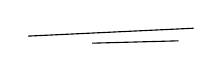
\begin{tikzpicture}\draw (0,0) -- (2.1,.10);\draw (.81,-.09) -- (1.91,-.06);\end{tikzpicture}}

\uline{Prop} Soit $G\xrightarrow{\deleted{\unsure{\lambda|v}}u}H$ \deleted{\unsure{Si}} hom de groupes\deleted{, avec $G$ qu. cpt} Si $u$ est plat \inserted{(générisant)} en un p$^{\mathrm{t}}$, il est plat \deleted{(au \unsure{p. gén.})} \inserted{(\uline{univ} générisant)} \deleted{et \unsure{donc} \unsure{est} plat} ; \deleted{donc $u(G)$ stable par \deleted{spécialisation} générisation}

% slanted
\margin{Il faut un argument pour ``univ'' générisant.}
\deleted{\uline{Cor} Supposons \deleted{que $H$ \unsure{qu cpt} qu'il existe} qu'il existe un p$^{\mathrm{t}}$ maximal $x$ de $H$ tel que $G_x\ne\varnothing$ (p. ex. $u$ dominant et $G$ qu. cpt) Alors \deleted{\unsure{$X$}} \inserted{si $H$ est réduit,} $u$ est plat, \deleted{donc généris\unsure{ant} (donc générisant \ldots)} Si on \inserted{ne} suppose pas \deleted{\uline{\unsure{Prop}} Su} $H$ réduit, $u$ est générisant, \deleted{et} l'image \deleted{\unsure{de}} $u(H)$ est stable \inserted{en} par générisation et contient}

\uline{Cor} Conditions équivalentes sur $u$

\deleted{\unsure{ouvert|affine}} a) $u$ est \inserted{univ} générisant \quad---\quad a$'$) $u$ générisant en un point.

b) $\unsure{U(G)|u(G)}\supset \deleted{G}H_0$

c) $\exists$ un point maximal \inserted{$x$} de $G$ tel que $u^{-1}(x)\ne\varnothing$.

Sous ces conditions, $u(G)$ est stable par spécialisation \deleted{(donc \unsure{fermé si} $G$ qu. cpt)}\margin{\deleted{\unsure{et H l. t. f.}}}

\uline{Dém} a) $\Longrightarrow$ a$'$) connu, a$'$) $\Longleftrightarrow$ \unsure{b)|c)} \deleted{\illegible{1}} trivial, b) $\Longrightarrow$ c) trivial, prouvons c) $\longrightarrow$ b. Or $W=u(G)$ est stable \uline{par $\deleted{G}H_0$}, donc les $\varphi_x$ étant générisants, il est stable par spécialisation ; \deleted{\unsure{OK}} donc b) devient trivial.

% slanted
\margin{\deleted{\unsure{avec}} Est-il \uline{tjrs} vrai que $u(G)$ stable par spécialisation? Oui. Je prouve \unsure{que|pour} tt ss-ens. stable par mult (et sym.) $\to$ stable par \unsure{spécia|spéc.}}
\uline{Cor} Si $G$ qu. cpt, \deleted{\unsure{domination} de $H^{\unsure{\mathrm{red}|\mathrm{t}}}$ \unsure{sur}} \inserted{$\operatorname{Im}u$ est fermée}

\uline{Prop.} Si $G\longrightarrow H$ un mono, avec $G$, \deleted{$H$} de t. f, \inserted{$H$ l. t. f.} alors $u$ est une immersion fermée.

\figure{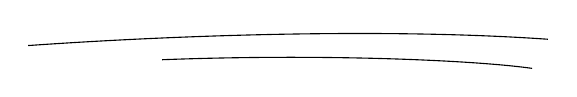
\begin{tikzpicture}\draw (0,0) .. controls (2,.14) and (4.6,.22) .. (6.6,.08);\draw (1.7,-.18) .. controls (3.8,-.10) and (5.7,-.19) .. (6.4,-.29);\end{tikzpicture}}

\diagram{$\displaystyle
\text{1)}\quad\left\{\begin{array}{l}
\text{Groupes discrets (\unsure{ev.|ev} tordus)}\\
\text{Groupes \unsure{profétales|profinis} \unsure{f.} }(\text{---})\\
\text{Groupes loc. cpts (tot. discontinus) (ev. tordus\unsure{)|{}}}
\end{array}\right.
\quad\left|\begin{array}{l}
\text{groupes}\\
\text{séparables}\\
\text{tot. discontinus}
\end{array}\right.$}

\[
\begin{aligned}
\unsure{\underline{\approx}|\cong}\quad &\text{groupes topologiques loc. compact}\\
 &\text{\inserted{tot. disc.} avec opérations \uline{continues} de }\pi\\
 &\pi\times G\longrightarrow G\quad\text{continue.}
\end{aligned}
\]

\diagram{$\displaystyle
\text{2)}\quad\begin{array}{l|l}
\text{\uline{Groupes connexes}} & \text{\uline{sur corps parfait} : Extension (can.)}\\
\text{\uline{\deleted{\unsure{s|S}}Séparables}} & \text{d'une VA par un groupe connexe}\\
\text{[sont qu. cpts]} & \text{lisse affine}\quad\Longleftrightarrow\quad \underset{\longleftarrow}{\lim} G_i,\\
& \text{les }G_i\text{ de type fini, partie abélienne}\\
& \text{de dim. majorée.}
\end{array}$}
% archive sheet number: 5

\scanpage{7}
\deleted{$X$ \unsure{loc.} de type fini sur}

\uline{Prop} Soit $X$ schéma \deleted{\unsure{localement|loc. noeth}} \deleted{\unsure{noethérien}} \inserted{régulier} sur corps $k$ \deleted{\unsure{de}} \uline{parfait}. Soit $k'$ une extension de $k$, supposons que \deleted{les ann} $X$ soit loc. de t. f. sur $k$ ou $k'$ ext. de type fini de $k$, de sorte que les anneaux locaux de $X_{k'}$ sont noeth. Alors $X_{k'}$ est régulier

$\unsure{\Updownarrow|\updownarrow}$\quad \uline{Corollaire} Soit $A$ un anneau local régulier sur $k$, $k'$ une extension de $k$. On suppose que $k'$ \deleted{est \unsure{loc.}} \inserted{ou $A$} de t. f. \deleted{\unsure{sur}} $k$., \deleted{\unsure{ou|{}} $A$ est de t. f. sur $k$} Alors $A\otimes_k k'$ est régulier.

% margin note written sideways
\margin{\uline{NB} Ne supposons pas $X$ \unsure{ess.|loc.} de t. f. sur $k$, \deleted{Il reste vrai que} \inserted{Alors si} $X$ est régulier pour tt extension \inserted{finie} \deleted{de la base} corps de base, \deleted{alors} pour tt $Y$ \unsure{ess.} de t. f. sur $S$, $Y$ régulier $\Longrightarrow X\times_kY$ \uline{régulier}. On dit que $X$ est géom régulier.}
% margin note written sideways
\margin{\unsure{Ex :|i.e. :} ext. de corps \uline{\unsure{alg.|sép.}}}
\uline{Prop} $X$ schéma \inserted{ess loc de t. f.} sur $k$, $k$, \unsure{ext:|est:} parfait. Conditions équivalentes

\diagram{\begin{tikzcd}[ampersand replacement=\&,row sep=.75em,column sep=.8em,execute at end picture={\draw ([xshift=-.75em]\tikzcdmatrixname-1-1.north west) .. controls +(0,-.55) and +(.24,0) .. ([xshift=-1.2em]\tikzcdmatrixname-2-1.west) .. controls +(.24,0) and +(0,.55) .. ([xshift=-.75em]\tikzcdmatrixname-4-1.south west);}]
\text{a)}\arrow[d,Rightarrow] \& {\forall\ \text{schéma }Y\text{ sur }k,\ Y\text{ régulier}\Longrightarrow X\times_kY\text{ régulier}}\\
\text{b)}\arrow[d,Rightarrow]\arrow[dd,bend right=37,Rightarrow] \& {\forall\ \text{ext. }k'/k,\ X_{k'}\text{ est régulier}}\\
\text{c)} \& {\deleted{\unsure{\forall}}\,X_{\unsure{k,|k'|\bar k}}\text{ régulier}}\\
\text{d)} \& {\forall\ \text{ext. finie }\deleted{\unsure{k'}}\ \text{radicielle }k'\text{ de }k,\ X_{k'}\text{ est régulier.}}
\end{tikzcd}}

\uline{Dém} b) $\to$ a) car si $A\to B$ hom$^{\mathrm t}$ local \inserted{plat} d'anneaux loc. noeth, $A$ régulier et $B/\unsure{\mathfrak m|m}B$ régulier \inserted{$\Rightarrow B$ régulier}

c) $\Rightarrow$ b) car si $\overset{\mathfrak m}{A}\to\overset{\mathfrak n}{B}$ hom local plat d'anneaux loc, noeth, \unsure{ds|des} $B$ régulier $\Rightarrow A$ régulier \ldots

d) $\Rightarrow$ c) par \unsure{principe} de limite.

\uline{Déf} On dit alors que $X$ est géom. régulier [ou \uline{lisse} sur $k$ si $X$ est loc. de t. f. sur $k$]

$X\deleted{\unsure{{}_k|{}_x}}$ \deleted{géom régulier}\deleted{lisse}\inserted{géom régulier} $\Longrightarrow X$ régulier. La réciproque est vraie pour tt $X$ sur $k$ (ou \unsure{seulement} pour tt $X=\operatorname{Spec}k'$, $k'$ ext. finie radicielle de $k$) ssi $k$ est parfait.

$X$, \deleted{géom rég}\deleted{lisse}\inserted{géom rég} $/k\Longleftrightarrow X_{k'}$ géom régulier sur $k'$

$X$ et $Y$ \deleted{géom réguliers}\deleted{lisse}\inserted{géom rég} sur $k$ $\Longrightarrow X\times_kY$ géom. réguliers sur $k$.

$X$ \deleted{\unsure{lisse}} géom. régulier/$\unsure{k|k'}$ en \uline{un point} $x\in X$ : $\operatorname{Loc}_x(X)$ est géom rég sur $k$ \inserted{ou $\underline O_{X,x}$ est géom rég}

On a les \unsure{faits|suits} analogues aux précédents.
\margin{\uline{NB} Si $k(x)$ est séparable sur $k$ régulier $\Rightarrow$ géom. rég.}

\deleted{\uline{Théorème} L'ens des p$^{\mathrm{ts}}$ de $X$, où $X$ est géom. régulier est ouvert. (On est ramené au cas où \deleted{\unsure{$X$}} $k$ est parfait \unsure{(i.e.|(} $=$ \unsure{rég.|Alg.} class).)}

\uline{Prop}\inserted{(Critère jacobien)} $X$ \inserted{loc de t f sur $k$} est \deleted{géom régulier}\inserted{lisse} en $x\in X$ ssi il existe un \inserted{entier $n\geq0$ et} morphisme $f:U_{\unsure{u|v|\smile}}\longrightarrow{\unsure{\mathbb E|E}}^{\unsure{n|h}}_k$ ($U$ vois. ouvert de $x$) tel que $f$ soit ``étale'' en $x$, i.e. [loc. en prés. finie] plat et à fibres étales

\uline{Corollaire} L'ens des p$^{\mathrm{ts}}$ où $X$ est \deleted{géom} lisse sur $k$ est ouvert.
% archive sheet number: 6

\scanpage{8}

\uline{Corollaire.} Cet \unsure{ouv|ouv.} est dense \unsure{ssi|ses} pour \unsure{tout|tt} pt \uline{maximal} $x\in X$, $\underline O_{X,x}$ est réduit et $k(x)$ est une extension \uline{séparable} de $k$ $[\Leftrightarrow$ \inserted{\unsure{au cas une|au cas d'une} ext. de \unsure{t.|T.} f.} extension étale d'une extension \unsure{transcend.te|transcendante|transcend. ou} pure$]$

\uline{Corollaire} Si $k$ est parfait, l'ens des pts où $X$ est lisse est un ouvert dense.

\uline{NB} On a un \unsure{réslt|rés\textsuperscript{t}} analogue pour la \uline{normalité géométrique}, sans condition de finitude. Si $X$ est \deleted{\unsure{géom normal|géom norm}} \inserted{loc de} t. f. sur $k$, l'ens des pts où $X$ est géom normal sur $k$ est ouvert, \inserted{et dense si $k$ est parfait} [Une extension d'un corps est géom normale ssi elle est séparable)

\figure{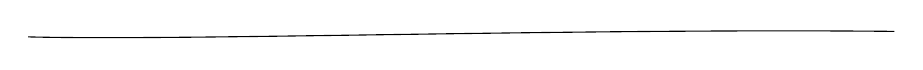
\begin{tikzpicture}\draw (0,0) .. controls (2,-.05) and (7,.11) .. (11,.07);\end{tikzpicture}}

\uline{Proposition} $G$ groupe sur corps $k$. Conditions équivalentes

\margin{marche aussi si $X$ un \deleted{\unsure{gpe|esp.}} \inserted{schéma} sur lequel $G$ opère et tel que \deleted{$G\times X\xrightarrow{\unsure{\pi|p}} X$} $G\times X\longrightarrow X\times X$ surjectif $(g,x)\longmapsto(gx,x)$ ($X$ essentiellement homogène)}% slanted

a) $G$ \deleted{\unsure{géom norm|géom. normal}} séparable $/k$ en un pt \qquad a$'$) $G$ sép. $/k$ \deleted{en un point}

b) $G$ géom normal sur $k$

c) (Si $G$ loc de t. f. sur $k$) $G$ lisse $/k$

On a évidemment \inserted{\unsure{c|c)} $\Rightarrow$} b) $\Rightarrow$ a$'$) \unsure{$\Rightarrow$|$\Longrightarrow$} a) \deleted{\unsure{$\Rightarrow$|$\Longrightarrow$} \unsure{b)|b)?}}.

\margin{\uline{NB} Si $G$ de t. f. sur $k$, alors $G$ \deleted{\unsure{re|ré}} \unsure{réduit|reduit} $\Rightarrow G$ sép.\unsure{?|!?} \deleted{(\unsure{est-ce que|et si pas|est-ce} le \unsure{$k$|$h$} \illegible{1} \unsure{stable dans|étant donné}}}% slanted

a) $\Rightarrow$ b) \qquad Soit $g\in G$, \deleted{un} pt maximal de $G$. \deleted{\unsure{géom|gén.}} \deleted{pour que $g$ \unsure{soit géom|soit} il \unsure{suffit que|suffit} $g$,} Alors $k(g)$ est une ext. séparable de $k$, donc $G$ est géom normal en $g$. \deleted{Donc, quitte \unsure{à faire une extension|à une extension} par descente on est ramené à \unsure{voir le cas|voir l'assert} pour $g$ rat. sur $k$.} \deleted{Soit $g'$ un pt maximal de $G$, on sait que $G$ est géom normal en $g'$; faisant une extension} Donc $G$ a \uline{un} pt $g$ où il est géom. normal. Prouvons qu'il en est de $=$ pour tt autre pt $g'$. Par ext. de la base, on est ramené au cas où $g$, $g'$ rat $/k$. Mais alors ils sont conjugués par translation !

b) $\Rightarrow$ a) \qquad \unsure{Est.|Ex.} en démonstration.

\uline{Corollaire 1} Soit $k$ parfait. Alors $G_{\text{\unsure{red|réd}}}$ est géom normal \unsure{$\bar k$|$k$|$\bar B$} (resp. lisse, si $G$ est loc. de t. f. sur $k$)

% archive sheet number: 7

